% !TeX program = xelatex
\documentclass[UTF8,a4paper,11pt,fontset=windows]{ctexart}
\usepackage[left=18mm,right=18mm,top=16mm,bottom=17mm,headheight=14pt]{geometry}
\usepackage{amsmath,amssymb,array,booktabs,longtable,needspace,fancyhdr,xcolor,tikz}
\usepackage[hidelinks]{hyperref}
\setlength{\parindent}{0pt}\setlength{\parskip}{3pt}\linespread{1.1}
\setlength{\emergencystretch}{2em}\raggedbottom
\pagestyle{fancy}\fancyhf{}\renewcommand{\headrulewidth}{0pt}
\fancyfoot[C]{\small\PaperName\quad 第\thepage 页}
\newcommand{\R}{\mathbb R}
\newcommand{\blank}{\underline{\hspace{2.9cm}}}
\newcommand{\src}[1]{\par{\scriptsize\color{black!65}教材改编出处：#1。}\par}
\newcommand{\q}[2]{\par\Needspace{4\baselineskip}\textbf{#1.}\ #2}
\newcommand{\subq}[2]{\par\Needspace{2\baselineskip}（#1）#2}
\newcommand{\opts}[4]{\par\begin{tabular*}{\linewidth}{@{}p{.48\linewidth}@{\extracolsep{\fill}}p{.48\linewidth}@{}}A. #1&B. #2\\C. #3&D. #4\end{tabular*}\par}
\newcommand{\optsfour}[4]{\par\begin{tabular*}{\linewidth}{@{}p{.235\linewidth}@{\extracolsep{\fill}}p{.235\linewidth}p{.235\linewidth}p{.235\linewidth}@{}}A. #1&B. #2&C. #3&D. #4\end{tabular*}\par}
\newcommand{\parttitle}[1]{\par\Needspace{4\baselineskip}{\bfseries #1}\par}
\newcommand{\work}[1]{\par\vspace*{#1}}
\newcommand{\ans}[2]{\par\Needspace{4\baselineskip}\textbf{第#1题}\quad #2\par}
\newcommand{\readinggraph}{\begin{center}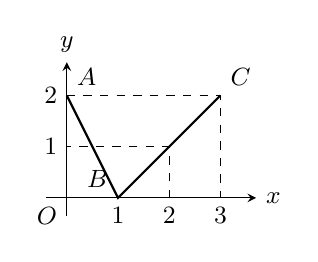
\begin{tikzpicture}[x=.65cm,y=.65cm,>=stealth,font=\small]
\draw[->](-.4,0)--(3.7,0)node[right]{$x$};\draw[->](0,-.35)--(0,2.65)node[above]{$y$};
\draw[thick](0,2)node[above right]{$A$}--(1,0)node[above left]{$B$}--(3,2)node[above right]{$C$};
\draw[dashed](0,2)--(3,2)--(3,0);\draw[dashed](2,0)--(2,1)--(0,1);
\node[below left]at(0,0){$O$};\foreach \x in {1,2,3}\node[below]at(\x,0){$\x$};
\foreach \y in {1,2}\node[left]at(0,\y){$\y$};\end{tikzpicture}\end{center}}
\renewcommand{\arraystretch}{1.2}

\newcommand{\PaperName}{B卷参考答案与评分}
\begin{document}
\begin{center}{\Large\bfseries 高一数学期中教材改编练习卷（B）}\\[2mm]参考答案、评分细则与教材出处\end{center}
单选、填空每题5分；多选全对6分，部分选对且无错项3分，含错项或未选0分。以下评分为本练习卷统一约定；解答题其他正确解法按相应步骤给分。
\parttitle{答案速查}\begin{center}\begin{tabular}{c|cccccccc}\toprule 题号&1&2&3&4&5&6&7&8\\答案&C&B&A&D&C&B&A&D\\\bottomrule\end{tabular}\par\smallskip\begin{tabular}{c|cccccc}\toprule 题号&9&10&11&12&13&14\\答案&AC&AB&BCD&$(-\infty,-1]$&$1$&$f(-2)<f(1)<f(3)$\\\bottomrule\end{tabular}\end{center}
\parttitle{单项选择题解析}
\ans{1}{\textbf{C}。并集包括两个集合中出现的全部元素，结果为 $\{0,1,2,3,4\}$，重复元素只写一次。}
\ans{2}{\textbf{B}。$x=3$ 能推出 $x^2=9$；$x^2=9$ 不一定推出 $x=3$，如 $x=-3$。故前者为后者的必要而不充分条件。}
\ans{3}{\textbf{A}。量词由全称改为存在，范围保持 $\R$，$\ge$ 的否定是 $<$。原命题本身的真假不改变否定形式。}
\ans{4}{\textbf{D}。$a^2+b^2\ge2ab=18$，当且仅当 $a=b=3$ 时取等号，满足约束。}
\ans{5}{\textbf{C}。A在0无定义，B在 $-1$ 无实数值，D在 $-1$ 的像为 $-2\notin B$；C在A上处处有唯一像，且均属于B。}
\ans{6}{\textbf{B}。根式要求 $x\ge-1$，分母要求 $x\ne\pm2$；其中 $-2$ 已不在前一范围中，故定义域为 $[-1,2)\cup(2,+\infty)$。}
\ans{7}{\textbf{A}。由偶性 $f(-3)=f(3)=9-12+1=-2$。}
\ans{8}{\textbf{D}。开口向下，递减区间为 $[a,+\infty)$。给定区间须在对称轴右侧，故 $a\le2$，端点可取。}
\parttitle{多项选择题与填空题解析}
\ans{9}{\textbf{AC}。A：$(1/a)-(1/b)=(b-a)/(ab)>0$。B：$|a|>|b|$，故平方后应为 $a^2>b^2$。C：除以负数b使不等号反向，$a/b>1$。D：取相反数后应为 $-a>-b$。}
\ans{10}{\textbf{AB}。$f(x)\ge4$，等号当且仅当 $x=2$。若 $0<x_1<x_2\le2$，则 $f(x_2)-f(x_1)=(x_2-x_1)(1-4/(x_1x_2))<0$，故在 $(0,2]$ 上递减。$f(1)=f(4)=5$，故C错误；最小值在2取得，D错误。}
\ans{11}{\textbf{BCD}。由 $f(2)=2f(1)=6$ 得 $f(1)=3$，A错误。令 $x=y=0$ 得 $f(0)=0$；令 $y=-x$ 得奇性；$f(6)=3f(2)=18$。故B、C、D正确。无需假设f在实数域上必为线性函数。}
\ans{12}{\textbf{$(-\infty,-1]$}。$-x^2+2x+k=-(x-1)^2+k+1$，最大值为 $k+1$。要求最大值不超过0，故 $k\le-1$。}
\ans{13}{\textbf{$1$}。先用第一段得 $f(-1)=1$，再用第二段得 $f(1)=1$。}
\ans{14}{\textbf{$f(-2)<f(1)<f(3)$}。奇性给出 $f(0)=0$；由正半轴含0的严格递增性得 $f(2)>0$，故 $f(-2)<0<f(1)<f(3)$。这里不能省略区间包含0的条件。}

\newpage
\parttitle{解答题解析与分步评分}
\ans{15}{（15分）\subq{1}{$A\cap B=[1,5)$（3分），$A\cup B=[-2,+\infty)$（3分），$\complement_U A=(-\infty,-2)\cup[5,+\infty)$（3分）。}\subq{2}{当 $t\ge5$ 时，B所有元素均不在A中（3分）；当 $t<5$ 时，可在 $[\max\{-2,t\},5)$ 中取到公共元素，因此不满足。故 $t\in[5,+\infty)$（3分）。}}
\src{p.13，习题1.1第9题；p.13，习题1.1第16题}
\ans{16}{（15分）\subq{1}{原式等价于 $(x+1)(x-4)<0$（3分），故解集为 $(-1,4)$（3分）。}\subq{2}{原式等价于 $(x-m)(x-2)\ge0$（3分）。当 $m<2$ 时，解集为 $(-\infty,m]\cup[2,+\infty)$（2分）；当 $m=2$ 时，解集为 $\R$（2分）；当 $m>2$ 时，解集为 $(-\infty,2]\cup[m,+\infty)$（2分）。}}
\src{p.59，习题2.3第4题；p.59，习题2.3第8题}
\ans{17}{（17分）\subq{1}{$f(0)=0$（2分），$f(-2)=-f(2)=-8$（2分）。}\subq{2}{当 $x<0$ 时 $-x>0$，$f(-x)=x^2-2x$（2分）；由奇性得 $f(x)=-x^2+2x$（3分）。}\subq{3}{任取 $x_1<x_2$（1分）。若 $0\le x_1<x_2$，则 $f(x_2)-f(x_1)=(x_2-x_1)(x_1+x_2+2)>0$（2分）。若 $x_1<x_2\le0$，则差为 $(x_2-x_1)(2-x_1-x_2)>0$（2分）。若 $x_1<0<x_2$，由解析式知 $f(x_1)<0<f(x_2)$（2分）。三类覆盖所有情形，故f在 $\R$ 上严格递增（1分）。}}
\src{p.86，习题3.2第6题；p.86，习题3.2第7题}
\ans{18}{（17分）\subq{1}{$16^{3/4}=8$（2分），$8^{-2/3}=1/4$，故原式为 $33/4$（2分）。}\subq{2}{由 $8^\alpha=2=8^{1/3}$ 得 $\alpha=1/3$（2分），故 $f(x)=\sqrt[3]x$（1分），定义域为 $\R$（2分）。}\subq{3}{$\sqrt[3]{-x}=-\sqrt[3]x$，且定义域对称，故为奇函数（2分）；在 $\R$ 上严格递增（2分）。任取 $0<x_1<x_2$，令 $u=\sqrt[3]{x_1},v=\sqrt[3]{x_2}$（1分），则 $v-u=(x_2-x_1)/(v^2+uv+u^2)>0$（2分），故正半轴上严格递增（1分）。所列全实数区间也成立：负半轴由奇性、跨零点由符号判断。}}
\src{p.104，习题4.1第4题；p.104，习题4.1第8题}
\ans{19}{（13分）\subq{1}{$f(0)=a=2$（3分）。}\subq{2}{底数大于1，外层指数函数递增；$|2x+1|$ 在 $(-\infty,-1/2]$ 上递减，在 $[-1/2,+\infty)$ 上递增，所以f在这两个区间分别递减、递增（各2分）。指数可取任意非负实数，故值域为 $[1,+\infty)$（2分）。}\subq{3}{原式等价于 $|2x+1|\le3$（2分），解得 $-2\le x\le1$，故解集为 $[-2,1]$（2分）。}}
\src{p.114，习题4.2第11题}

\newpage
\parttitle{命题结构与教材改编记录}
本卷只使用教材第1至3章及第4章4.1至4.2的例题、习题和练习作为母题。集合与逻辑30分，不等式31分，函数概念与性质59分，幂函数与指数函数30分；合计150分。
\par 主考点归类：集合1、15题共20分，逻辑2、3题共10分；基本不等式4题5分、不等式性质9题6分、恒成立12题5分、二次不等式16题15分；函数概念5、6、13题共15分，函数性质7、8、10、11、14、17题共44分；幂函数18题17分、指数函数19题13分。综合题允许知识交叉，归类用于统计，不将同一分数重复计入。
\par 教材页码指印刷页，正文PDF页序为印刷页加7。下列ID均可在教材题库中检索，改编题的答案已另行重算，不能直接套用母题答案。
\par 未特别注明的改编均为更换数据与设问、保留教材母题的概念结构。逐题目标、预期方法、易错点及评价方式另见随附“命题细目与教材出处.csv”。
\small\begin{longtable}{@{}p{.045\linewidth}p{.925\linewidth}@{}}\toprule 题号&教材母题与改编说明\\\midrule\endhead
1 & p.13，习题1.1第8题（PDF第20页）\newline{\scriptsize\ttfamily\detokenize{XJ-B1-C01-HW-P013-Y0307}}\\[3pt]
2 & p.18，例5（PDF第25页）\newline{\scriptsize\ttfamily\detokenize{XJ-B1-C01-EX-P018-Y0491}}\\[3pt]
3 & p.23，页首练习（PDF第30页）\newline{\scriptsize\ttfamily\detokenize{XJ-B1-C01-PR-P023-Y0176}}\\[3pt]
4 & p.43，习题2.1第5题（PDF第50页）\newline{\scriptsize\ttfamily\detokenize{XJ-B1-C02-HW-P043-Y1062}}\\[3pt]
5 & p.67，练习第1题（PDF第74页）\newline{\scriptsize\ttfamily\detokenize{XJ-B1-C03-PR-P067-Y0874}}\\[3pt]
6 & p.77，习题3.1第4题（PDF第84页）\newline{\scriptsize\ttfamily\detokenize{XJ-B1-C03-HW-P077-Y0286}}\\[3pt]
7 & p.86，习题3.2第7题（PDF第93页）\newline{\scriptsize\ttfamily\detokenize{XJ-B1-C03-HW-P086-Y0288}}\\[3pt]
8 & p.82，练习第3题（PDF第89页）\newline{\scriptsize\ttfamily\detokenize{XJ-B1-C03-PR-P082-Y1536}}\\[3pt]
9 & p.43，习题2.1第3题（PDF第50页）\newline{\scriptsize\ttfamily\detokenize{XJ-B1-C02-HW-P043-Y0634}}\\[3pt]
10 & p.81，例2（PDF第88页）\newline{\scriptsize\ttfamily\detokenize{XJ-B1-C03-EX-P081-Y1313}}\\[3pt]
11 & p.91，复习题第12题（PDF第98页）\newline{\scriptsize\ttfamily\detokenize{XJ-B1-C03-RV-P091-Y0650}}\\[3pt]
12 & p.55，例5（PDF第62页）\newline{\scriptsize\ttfamily\detokenize{XJ-B1-C02-EX-P055-Y0177}}\\[3pt]
13 & p.76，练习第2题（PDF第83页）\newline{\scriptsize\ttfamily\detokenize{XJ-B1-C03-PR-P076-Y0364}}\\[3pt]
14 & p.86，习题3.2第11题（PDF第93页）\newline{\scriptsize\ttfamily\detokenize{XJ-B1-C03-HW-P086-Y1034}}\newline 改编：把教材偶函数、减函数改为奇函数、在含0的正半轴上递增，并更换比较点。\\[3pt]
15 & p.13，习题1.1第9题（PDF第20页）；p.13，习题1.1第16题（PDF第20页）\newline{\scriptsize\ttfamily\detokenize{XJ-B1-C01-HW-P013-Y0433 / XJ-B1-C01-HW-P013-Y1442}}\\[3pt]
16 & p.59，习题2.3第4题（PDF第66页）；p.59，习题2.3第8题（PDF第66页）\newline{\scriptsize\ttfamily\detokenize{XJ-B1-C02-HW-P059-Y0221 / XJ-B1-C02-HW-P059-Y0874}}\\[3pt]
17 & p.86，习题3.2第6题（PDF第93页）；p.86，习题3.2第7题（PDF第93页）\newline{\scriptsize\ttfamily\detokenize{XJ-B1-C03-HW-P086-Y0231 / XJ-B1-C03-HW-P086-Y0288}}\newline 改编：融合教材奇函数求值与对称延拓母题，更换系数，并增加跨零点的定义证明。\\[3pt]
18 & p.104，习题4.1第4题（PDF第111页）；p.104，习题4.1第8题（PDF第111页）\newline{\scriptsize\ttfamily\detokenize{XJ-B1-C04-HW-P104-Y0874 / XJ-B1-C04-HW-P104-Y1494}}\\[3pt]
19 & p.114，习题4.2第11题（PDF第121页）\newline{\scriptsize\ttfamily\detokenize{XJ-B1-C04-HW-P114-Y1038}}\\[3pt]
\bottomrule\end{longtable}\normalsize
\par\textbf{评价与复习建议：}客观题逐项判断，填空题核对端点和可取性；解答题按列式、推理、分类完整性及结论评分。第17、18题重点观察能否从定义出发说明理由。上述难度与错误仅为教学预判，未经过班级试测，不预设均分或达标率。
\end{document}
